\documentclass[border=3pt]{standalone}
\usepackage{tikz}
\usetikzlibrary {angles,calc,quotes}

\begin{document}
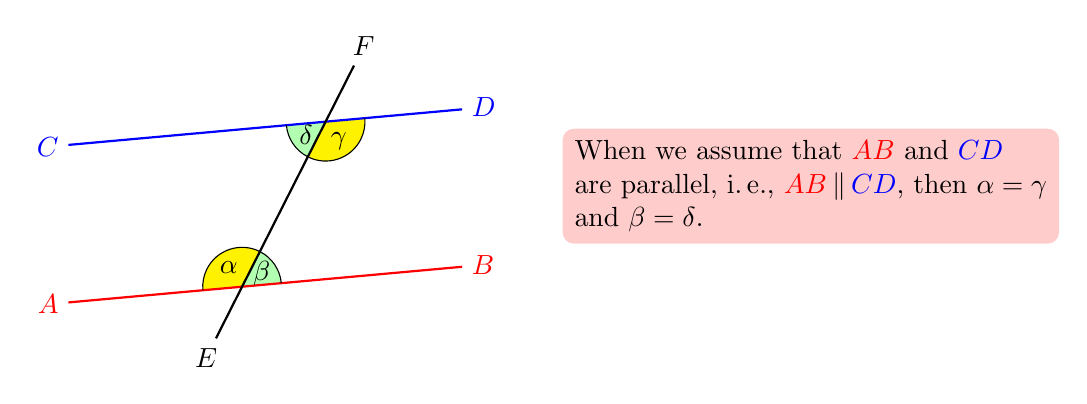
\begin{tikzpicture}

  \node (A) at (-2,0)     [red,left]   {$A$};
  \node (B) at ( 3,.5)    [red,right]  {$B$};
  \node (C) at (-2,2)     [blue,left]  {$C$};
  \node (D) at ( 3,2.5)   [blue,right] {$D$};
  \node (E) at (60:-5mm)  [below]      {$E$};
  \node (F) at (60:3.5cm) [above]      {$F$};

  \coordinate (X) at (intersection cs:first line={(A)--(B)}, second line={(E)--(F)});
  \coordinate (Y) at (intersection cs:first line={(C)--(D)}, second line={(E)--(F)});

  \path
    (A) edge [red, thick]  (B)
    (C) edge [blue, thick] (D)
    (E) edge [thick]       (F)
      pic ["$\alpha$", draw, fill=yellow]   {angle = F--X--A}
      pic ["$\beta$",  draw, fill=green!30] {angle = B--X--F}
      pic ["$\gamma$", draw, fill=yellow]   {angle = E--Y--D}
      pic ["$\delta$", draw, fill=green!30] {angle = C--Y--E};

  \node at ($ (D)!.5!(B) $) [right=1cm,text width=6cm,rounded corners,fill=red!20,inner sep=1ex]
    {
      When we assume that $\color{red}AB$ and $\color{blue}CD$ are
      parallel, i.\,e., ${\color{red}AB} \mathbin{\|} \color{blue}CD$,
      then $\alpha = \gamma$ and $\beta = \delta$.
    };
\end{tikzpicture}

\end{document}